\en{Let $ABC$ be an acute triangle with $AB = AC$ and let $D$ be a point on the side $BC$. The circle with centre $D$ passing through $C$ intersects the circumcircle of $ABD$ in $P$ and $Q$, where $Q$ is the point closer to $B$. The line $BQ$ intersects $AD$ in $X$ and $AC$ in $Y$. Prove that $PDXY$ is cyclic.

\textbf{Solution:} We first claim that $P\in AC$. Indeed, let $P'$ be the second intersection between the circle centered at $D$ and $AC$. Then
\[
\angle ABD= \angle ABC=\angle ACB=\angle P'CD=180^\circ- \angle AP'D.
\]
so that $ABDP'$ is cyclic. This implies that $P=P'$, in particular $P\in AC$. As $DP=DQ$, the arcs $DP$ and $DQ$ subtend angles of same measure on the circle $(APDQB)$, so that $\angle QBD=\angle PAD$. Hence, $\Delta DBX$ and $\Delta DAC$ are similar (alternatively $ABXC$ is cyclic), implying that $\angle DXB=\angle DCA$. This concludes the problem, as we wanted to prove that
\[
\angle DPY=\angle DPC=\angle DCP=\angle DCA=\angle DXB=180^\circ -\angle DXY.
\]

\begin{center}
    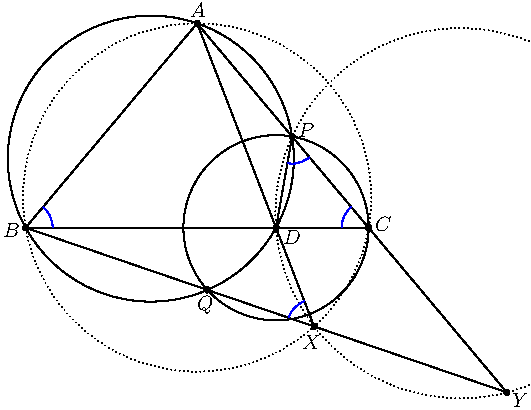
\includegraphics[scale=1]{2021/Final round/MasterSolution/Solutions/f2fig.pdf}
\end{center}

\textbf{Marking scheme}
\begin{itemize}
    \item 1P: Claim that $P$ lies on $AC$.
    
    \item 2P: Prove that $P$ lies on $AC$.
    
    \item 2P: Prove that $\angle QBD=\angle PAD$.
    
    \item 2P: Conclude. (Proving that $ABXC$ cyclic is enough to end the problem gives these two points for example)
\end{itemize}
}

